\chapter{Machine architecture for software designers}
As software designers, we may work with different mental models of the hardware
that run our programs. Particularly performance-conscious designers may be
concerned with the access speeds of CPU registers vs CPU cache. C programmers
may think of main memory and cache as a single, contiguous address-space that
they can manipulate freely. And if they wish, java programmers may ignore even
the existence of the memory hierarchy altogether, and simply think about objects
and their relationships.

The purpose of this section is to help multicore-software designers understand the
workings of the memory hierarchy. To that end, I describe the memory hierarchy
in a manner that is abstract enough to be useful (and understandable) for the
non-hardware oriented software designer, but detailed enough to explain the
performance characteristics of e.g. false sharing.

\section{Model of the computer}
We will work with a simplified model of a computer, consisting of the following
components:

\begin{itemize}
	\item CPU cores, each with their own registers. A core executes a single
		thread at a time, or more if it uses hyper-threading.
	\item Individual CPUs, each of which may contain multiple individual cores.
	\item Per-CPU cache hierarchies, with multiple layers of cache,
		some of which are shared between multiple cores.
	\item Main memory (colloquially RAM), shared between all CPUs.
\end{itemize}

\mynote{add diagram of main-memory $\to$ L3-L1 cache $\to$ cpu cores}

This model excludes many aspects of real computers. Such as: Hard drives,
network interfaces, the buses that transfer data between hardware components,
and address-translation hardware such as translation lookaside buffers. Each of
these may or may not have their own interesting multicore-performance
characteristics, that we shall simply ignore.

In this model, main memory is the slowest resource we work with. As we shall see
in section \ref{sec:experiments}, \mynote{I'm still not sure where the cyclic
reads plots will end up (here, experiment section, or "memory operations are
expensive" section); get back to this} reading from main memory takes on the
order of 35-140 nanoseconds, whereas reading from L1 cache can be done in 1-4
nanoseconds. It follows directly from this fact that the cache-friendliness of a
program can significantly impact performance: If a program performs a billion
reads, this is the difference between a second and a few minutes.

So why not built larger caches? As commented earlier, larger caches generally
mean longer access times. Going to extremes, \citeauthor{mckenney} \cite{mckenney} notes that in order
to access storage within the time of a single 5GHz CPU-clock cycle, the storage
can be no more than 3 centimeters away from the CPU core, or we would have to
transfer the data faster than the speed of light. Furthermore; we do not (yet)
use light to transfer information between the components of a computer. We use
low-voltage electricity, which is (according to \cite{mckenney}) about 3-30
times slower.

\section{Main memory}
The main memory functions as a kind of backbone of the memory hierarchy. It is
large (often in the tens of gigabytes), and when working with high-level
languages, we tend to think about the entire memory
hierarchy in terms of how the main memory works: A contiguous storage space,
divided into fixed chunks of equal size, each of which can be
accessed individually using fixed-width addresses. This "fixed-width" is
generally what is meant when we say an architecture is "x-bit": A 64-bit
architecture uses memory addresses that are 64-bit long, and has 64-bit long
words. This terminology is \textit{not} consistent and some architectures may
have word sizes that are not the same as the address size. Furthermore,
definitions of the terms "word" and "address" that are both precise and useful
have proven elusive: Existing 64-bit architectures do not use the full 64-bit
address space, and may impose requirements on how the unused bits are set.
Virtual addresses, as used by programmers, are translated to physical addresses
using complicated techniques that may be implemented both in circuitry and in
the operating system. The term "word" seems to simply mean "some useful number
on a given architecture". Useful because memory addresses, CPU instructions, CPU
registers, integers, floating point numbers, and the amount of memory that is
described by a single address are \textit{typically} the size of a word, or some
multiple or fraction of it. For example, x86-64 has 64-bit words and addresses,
but some implementations support 80- or even 128-bit floating point operations.

On x86 (and x86-64), an address refers to an individual byte, not a word. However,
reading from an address in main memory does not necessarily mean reading just
that one byte. Though it not always the case, we generally consider the word
size to be the unit of memory operations.

\section{CPU caches}
Regardless of how the software designer thinks of memory, the CPU cache is not
generally a part of their interface: cache access happens transparently as we
access the main memory. It is not however transparent with
respect to performance, and cache-sympathetic software design can yield
significant performance gains. A famous example of this is found in the 2012
\texttt{GoingNative} keynote by \citeauthor{stroustrup} \cite{stroustrup}, in
which he explains that insertion into linked lists is much slower than
insertion into arrays/vectors, because of the unpredictable memory access
pattern exhibited by traversing a linked list. In this section we take a look
at the performance characteristics of CPU caches, and see that cache-friendly
design in multicore programming is radically different from cache-friendly
design in single-core programming.

A word of caution:
Since the cache is mostly invisible to software designers, hardware designers
have a lot of freedom when designing them. This makes it difficult to model and
reason about cache-behaviour across platforms. This section gives an overview
of cache hardware that applies to most modern, general-purpose hardware,
including x86 and x86-64 implementations. For a more comprehensive outline of
modern memory-hardware, chapters 2, 3, and 6 of
\cite{whatprogrammersshouldknow} should be of help. However, as is usually the
case with hardware performance, the best way to determine how a program
performs with respect to the cache is to run benchmarks on the exact platform
it will run on.

\subsection{What is cached and how} The cache works by storing copies
of information from main memory. That way, the cache provides faster access to
memory contents we expect to access in the future.

We could think of caches as general key-value stores, associating memory
addresses with cached values. Such a cache could let us cache values for any
set of memory locations we would like, subject only to the space constraints of
the cache. This type of cache (called \textit{fully associative}) scales
poorly as we would have to store the memory addresses in addition to the cached
values. Furthermore, any read or write operation must search the cache for the
relevant memory address. While this may sound simple enough to software
designers, cache behaviours are implemented as circuitry. For these reasons,
large caches -- such as the multi-kilobyte L1 caches closest to the CPU cores
-- are not implemented this way. Instead, set-associative caches are used
\cite{whatprogrammersshouldknow} \cite{mckenny-barriers}.

A set-associative cache is like is a hardware hash table with probing and
fixed-sized buckets -- or "sets". Each memory address hashes to a specific set,
and each set can contain a fixed number of entries, called "ways". The hash
function simply takes a fixed number of the least significant bits of the
address. This eliminates the need for storing the full memory address of each
cache entry: Part of the address is implied by the set used. The need to search
the full cache is similarly eliminated: The hardware now only needs to search
within a single set.

The downside is, that unlike fully associative caches, set-associative caches
cannot store an arbitrary set of entries. In a 2-way set-associative cache, two
entries whose addresses hash to the same bucket can be stored at a time. If a
new entry hashes to the same bucket, one of the two first will be evicted from
the cache, regardless of how much free space is in the other buckets. According
to \citeauthor{whatprogrammersshouldknow}, typical CPUs in 2007 used
associativity levels of up to 24 ways for L2 and larger caches, and 8 ways for L1
\cite{whatprogrammersshouldknow}. Intel's optimization manual
\cite{inteloptimize} indicates that CPUs using their Skylake microarchitecture
(from 2015) use 8 ways in L1, 4 ways in L2, and up to 16 ways in L3, so the
2007 figures appear to be current.

The storage in each way in a set is called a cache-line. The cache-line
size can be thought of as a unit size of cache operations. Most, if not all, of
Intel's x86-64 architectures use 64-byte cache-lines\cite{inteloptimize}.

In summary, 

\mynote{cache-line def/explanation goes here (or to the end of subsect). Comment sim/dif to mem access
word/byte granularity and (lack of) cache associativity compared to mem}

Several things can cause information to be copied in cache. In general, all
reads by a CPU core from main memory \textit{may} be stored in cache, under the
assumption that having accessed it once, the data will likely be accessed
again soon after. Similarly, the cache works as a buffer for writes to main
memory: When a CPU writes a value to a memory address the value is actually
stored in the CPU's own cache. The cache will then write the value back to main
memory (or to a cache higher up in the hierarchy) at a later time. The contents of main memory may also be cached by clever
prefetch mechanisms that anticipate future accesses. For example, iterating over
the elements of an array creates a memory access-pattern (also know as a
"stride") that is easily predictable. It may help to think of such access
patterns as a function $f(n) = \ldots$, where $n$ is the number of accesses we
have already made, and $f(n)$ is the next address we want to access. The stride
of reading every third element from an array can then be described by the linear
function $f(n) = 3n$ (ignoring the complexities of virtual memory, and the array
base-pointer). The first access is to address $f(0) = 0$, the second to $f(1) =
3$, etc. Individual caches have associated prefetch-hardware that essentially
performs regression-analysis of actual memory accesses in order to guess the
constants of the stride function and perform reads before they are requested.
Modern commodity hardware can generally predict strides that are linear
function, not just sequential ones. Some hardware platforms (e.g. x64 and x86-64)
also provide instructions for prefetching; letting software designers prefetch
manually if the hardware prefetch mechanism are
unsatisfactory\cite{whatprogrammersshouldknow}.

\subsection{Data sharing}
The fact that writes are buffered in the caches is our first hint that
multi-core programming is non-trivial. As different CPU cores may store copies
of data from main memory in their own caches (and in registers as well), it is
possible for different cores to have different ideas of what the value stored at
a certain memory address is.

\mynote{add diagram showing the same "variable" differing in
main-mem/cpu0-cache/cpu1-cache/cpu1-registers}

This incoherence between what different cores see as the memory contents at a
certain address, and the way it is solved in hardware, is what gives rise to the
problem of false sharing.

\mynote{Continue writing: write-back caches (as described by drepper), MESI
state states, store-buffers and invalidation queues (explanation of
false-sharing impact)}

\begin{figure}[hbpt]
	\graphicspath{{plots/}}
	\begin{subfigure}{1\textwidth}
		% GNUPLOT: LaTeX picture with Postscript
\begingroup
  \makeatletter
  \providecommand\color[2][]{%
    \GenericError{(gnuplot) \space\space\space\@spaces}{%
      Package color not loaded in conjunction with
      terminal option `colourtext'%
    }{See the gnuplot documentation for explanation.%
    }{Either use 'blacktext' in gnuplot or load the package
      color.sty in LaTeX.}%
    \renewcommand\color[2][]{}%
  }%
  \providecommand\includegraphics[2][]{%
    \GenericError{(gnuplot) \space\space\space\@spaces}{%
      Package graphicx or graphics not loaded%
    }{See the gnuplot documentation for explanation.%
    }{The gnuplot epslatex terminal needs graphicx.sty or graphics.sty.}%
    \renewcommand\includegraphics[2][]{}%
  }%
  \providecommand\rotatebox[2]{#2}%
  \@ifundefined{ifGPcolor}{%
    \newif\ifGPcolor
    \GPcolorfalse
  }{}%
  \@ifundefined{ifGPblacktext}{%
    \newif\ifGPblacktext
    \GPblacktexttrue
  }{}%
  % define a \g@addto@macro without @ in the name:
  \let\gplgaddtomacro\g@addto@macro
  % define empty templates for all commands taking text:
  \gdef\gplbacktext{}%
  \gdef\gplfronttext{}%
  \makeatother
  \ifGPblacktext
    % no textcolor at all
    \def\colorrgb#1{}%
    \def\colorgray#1{}%
  \else
    % gray or color?
    \ifGPcolor
      \def\colorrgb#1{\color[rgb]{#1}}%
      \def\colorgray#1{\color[gray]{#1}}%
      \expandafter\def\csname LTw\endcsname{\color{white}}%
      \expandafter\def\csname LTb\endcsname{\color{black}}%
      \expandafter\def\csname LTa\endcsname{\color{black}}%
      \expandafter\def\csname LT0\endcsname{\color[rgb]{1,0,0}}%
      \expandafter\def\csname LT1\endcsname{\color[rgb]{0,1,0}}%
      \expandafter\def\csname LT2\endcsname{\color[rgb]{0,0,1}}%
      \expandafter\def\csname LT3\endcsname{\color[rgb]{1,0,1}}%
      \expandafter\def\csname LT4\endcsname{\color[rgb]{0,1,1}}%
      \expandafter\def\csname LT5\endcsname{\color[rgb]{1,1,0}}%
      \expandafter\def\csname LT6\endcsname{\color[rgb]{0,0,0}}%
      \expandafter\def\csname LT7\endcsname{\color[rgb]{1,0.3,0}}%
      \expandafter\def\csname LT8\endcsname{\color[rgb]{0.5,0.5,0.5}}%
    \else
      % gray
      \def\colorrgb#1{\color{black}}%
      \def\colorgray#1{\color[gray]{#1}}%
      \expandafter\def\csname LTw\endcsname{\color{white}}%
      \expandafter\def\csname LTb\endcsname{\color{black}}%
      \expandafter\def\csname LTa\endcsname{\color{black}}%
      \expandafter\def\csname LT0\endcsname{\color{black}}%
      \expandafter\def\csname LT1\endcsname{\color{black}}%
      \expandafter\def\csname LT2\endcsname{\color{black}}%
      \expandafter\def\csname LT3\endcsname{\color{black}}%
      \expandafter\def\csname LT4\endcsname{\color{black}}%
      \expandafter\def\csname LT5\endcsname{\color{black}}%
      \expandafter\def\csname LT6\endcsname{\color{black}}%
      \expandafter\def\csname LT7\endcsname{\color{black}}%
      \expandafter\def\csname LT8\endcsname{\color{black}}%
    \fi
  \fi
    \setlength{\unitlength}{0.0500bp}%
    \ifx\gptboxheight\undefined%
      \newlength{\gptboxheight}%
      \newlength{\gptboxwidth}%
      \newsavebox{\gptboxtext}%
    \fi%
    \setlength{\fboxrule}{0.5pt}%
    \setlength{\fboxsep}{1pt}%
\begin{picture}(7200.00,3880.80)%
    \gplgaddtomacro\gplbacktext{%
      \csname LTb\endcsname%%
      \put(528,500){\makebox(0,0)[r]{\strut{}$0$}}%
      \put(528,816){\makebox(0,0)[r]{\strut{}$2$}}%
      \put(528,1132){\makebox(0,0)[r]{\strut{}$4$}}%
      \put(528,1448){\makebox(0,0)[r]{\strut{}$6$}}%
      \put(528,1764){\makebox(0,0)[r]{\strut{}$8$}}%
      \put(528,2080){\makebox(0,0)[r]{\strut{}$10$}}%
      \put(528,2396){\makebox(0,0)[r]{\strut{}$12$}}%
      \put(528,2712){\makebox(0,0)[r]{\strut{}$14$}}%
      \put(528,3028){\makebox(0,0)[r]{\strut{}$16$}}%
      \put(528,3344){\makebox(0,0)[r]{\strut{}$18$}}%
      \put(528,3660){\makebox(0,0)[r]{\strut{}$20$}}%
      \put(752,368){\rotatebox{-45}{\makebox(0,0)[l]{\strut{}8}}}%
      \put(844,368){\rotatebox{-45}{\makebox(0,0)[l]{\strut{}16}}}%
      \put(1027,368){\rotatebox{-45}{\makebox(0,0)[l]{\strut{}32}}}%
      \put(1395,368){\rotatebox{-45}{\makebox(0,0)[l]{\strut{}64}}}%
      \put(2130,368){\rotatebox{-45}{\makebox(0,0)[l]{\strut{}128}}}%
      \put(3600,368){\rotatebox{-45}{\makebox(0,0)[l]{\strut{}256}}}%
      \put(6539,368){\rotatebox{-45}{\makebox(0,0)[l]{\strut{}512}}}%
    }%
    \gplgaddtomacro\gplfronttext{%
      \csname LTb\endcsname%%
      \put(5552,3487){\makebox(0,0)[r]{\strut{}readtimes-by-array-size}}%
      \csname LTb\endcsname%%
      \put(5552,3267){\makebox(0,0)[r]{\strut{}readtimes-by-array-size-padded}}%
      \csname LTb\endcsname%%
      \put(5552,3047){\makebox(0,0)[r]{\strut{}readtimes-by-array-size-desktop}}%
      \csname LTb\endcsname%%
      \put(5552,2827){\makebox(0,0)[r]{\strut{}readtimes-by-array-size-padded-desktop}}%
      \csname LTb\endcsname%%
      \put(5552,2607){\makebox(0,0)[r]{\strut{}readtimes-by-array-size-server}}%
      \csname LTb\endcsname%%
      \put(5552,2387){\makebox(0,0)[r]{\strut{}readtimes-by-array-size-padded-server}}%
    }%
    \gplbacktext
    \put(0,0){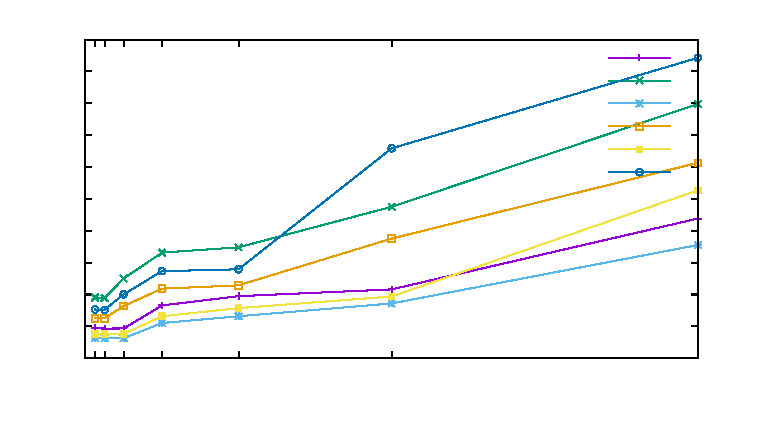
\includegraphics{readtimes}}%
    \gplfronttext
  \end{picture}%
\endgroup

	\end{subfigure}
	\begin{subfigure}{1\textwidth}
		% GNUPLOT: LaTeX picture with Postscript
\begingroup
  \makeatletter
  \providecommand\color[2][]{%
    \GenericError{(gnuplot) \space\space\space\@spaces}{%
      Package color not loaded in conjunction with
      terminal option `colourtext'%
    }{See the gnuplot documentation for explanation.%
    }{Either use 'blacktext' in gnuplot or load the package
      color.sty in LaTeX.}%
    \renewcommand\color[2][]{}%
  }%
  \providecommand\includegraphics[2][]{%
    \GenericError{(gnuplot) \space\space\space\@spaces}{%
      Package graphicx or graphics not loaded%
    }{See the gnuplot documentation for explanation.%
    }{The gnuplot epslatex terminal needs graphicx.sty or graphics.sty.}%
    \renewcommand\includegraphics[2][]{}%
  }%
  \providecommand\rotatebox[2]{#2}%
  \@ifundefined{ifGPcolor}{%
    \newif\ifGPcolor
    \GPcolorfalse
  }{}%
  \@ifundefined{ifGPblacktext}{%
    \newif\ifGPblacktext
    \GPblacktexttrue
  }{}%
  % define a \g@addto@macro without @ in the name:
  \let\gplgaddtomacro\g@addto@macro
  % define empty templates for all commands taking text:
  \gdef\gplbacktext{}%
  \gdef\gplfronttext{}%
  \makeatother
  \ifGPblacktext
    % no textcolor at all
    \def\colorrgb#1{}%
    \def\colorgray#1{}%
  \else
    % gray or color?
    \ifGPcolor
      \def\colorrgb#1{\color[rgb]{#1}}%
      \def\colorgray#1{\color[gray]{#1}}%
      \expandafter\def\csname LTw\endcsname{\color{white}}%
      \expandafter\def\csname LTb\endcsname{\color{black}}%
      \expandafter\def\csname LTa\endcsname{\color{black}}%
      \expandafter\def\csname LT0\endcsname{\color[rgb]{1,0,0}}%
      \expandafter\def\csname LT1\endcsname{\color[rgb]{0,1,0}}%
      \expandafter\def\csname LT2\endcsname{\color[rgb]{0,0,1}}%
      \expandafter\def\csname LT3\endcsname{\color[rgb]{1,0,1}}%
      \expandafter\def\csname LT4\endcsname{\color[rgb]{0,1,1}}%
      \expandafter\def\csname LT5\endcsname{\color[rgb]{1,1,0}}%
      \expandafter\def\csname LT6\endcsname{\color[rgb]{0,0,0}}%
      \expandafter\def\csname LT7\endcsname{\color[rgb]{1,0.3,0}}%
      \expandafter\def\csname LT8\endcsname{\color[rgb]{0.5,0.5,0.5}}%
    \else
      % gray
      \def\colorrgb#1{\color{black}}%
      \def\colorgray#1{\color[gray]{#1}}%
      \expandafter\def\csname LTw\endcsname{\color{white}}%
      \expandafter\def\csname LTb\endcsname{\color{black}}%
      \expandafter\def\csname LTa\endcsname{\color{black}}%
      \expandafter\def\csname LT0\endcsname{\color{black}}%
      \expandafter\def\csname LT1\endcsname{\color{black}}%
      \expandafter\def\csname LT2\endcsname{\color{black}}%
      \expandafter\def\csname LT3\endcsname{\color{black}}%
      \expandafter\def\csname LT4\endcsname{\color{black}}%
      \expandafter\def\csname LT5\endcsname{\color{black}}%
      \expandafter\def\csname LT6\endcsname{\color{black}}%
      \expandafter\def\csname LT7\endcsname{\color{black}}%
      \expandafter\def\csname LT8\endcsname{\color{black}}%
    \fi
  \fi
    \setlength{\unitlength}{0.0500bp}%
    \ifx\gptboxheight\undefined%
      \newlength{\gptboxheight}%
      \newlength{\gptboxwidth}%
      \newsavebox{\gptboxtext}%
    \fi%
    \setlength{\fboxrule}{0.5pt}%
    \setlength{\fboxsep}{1pt}%
\begin{picture}(7200.00,3780.00)%
    \gplgaddtomacro\gplbacktext{%
      \csname LTb\endcsname%%
      \put(528,593){\makebox(0,0)[r]{\strut{}$0$}}%
      \put(528,890){\makebox(0,0)[r]{\strut{}$5$}}%
      \put(528,1186){\makebox(0,0)[r]{\strut{}$10$}}%
      \put(528,1483){\makebox(0,0)[r]{\strut{}$15$}}%
      \put(528,1779){\makebox(0,0)[r]{\strut{}$20$}}%
      \put(528,2076){\makebox(0,0)[r]{\strut{}$25$}}%
      \put(528,2373){\makebox(0,0)[r]{\strut{}$30$}}%
      \put(528,2669){\makebox(0,0)[r]{\strut{}$35$}}%
      \put(528,2966){\makebox(0,0)[r]{\strut{}$40$}}%
      \put(528,3262){\makebox(0,0)[r]{\strut{}$45$}}%
      \put(528,3559){\makebox(0,0)[r]{\strut{}$50$}}%
      \put(660,461){\rotatebox{-45}{\makebox(0,0)[l]{\strut{}512}}}%
      \put(1052,461){\rotatebox{-45}{\makebox(0,0)[l]{\strut{}1024}}}%
      \put(1836,461){\rotatebox{-45}{\makebox(0,0)[l]{\strut{}2048}}}%
      \put(2620,461){\rotatebox{-45}{\makebox(0,0)[l]{\strut{}3072}}}%
      \put(3404,461){\rotatebox{-45}{\makebox(0,0)[l]{\strut{}4096}}}%
      \put(6539,461){\rotatebox{-45}{\makebox(0,0)[l]{\strut{}8192}}}%
    }%
    \gplgaddtomacro\gplfronttext{%
      \csname LTb\endcsname%%
      \put(5552,3386){\makebox(0,0)[r]{\strut{}i5}}%
      \csname LTb\endcsname%%
      \put(5552,3166){\makebox(0,0)[r]{\strut{}padded-i5}}%
      \csname LTb\endcsname%%
      \put(5552,2946){\makebox(0,0)[r]{\strut{}i7}}%
      \csname LTb\endcsname%%
      \put(5552,2726){\makebox(0,0)[r]{\strut{}padded-i7}}%
      \csname LTb\endcsname%%
      \put(5552,2506){\makebox(0,0)[r]{\strut{}Xeon}}%
      \csname LTb\endcsname%%
      \put(5552,2286){\makebox(0,0)[r]{\strut{}padded-Xeon}}%
    }%
    \gplbacktext
    \put(0,0){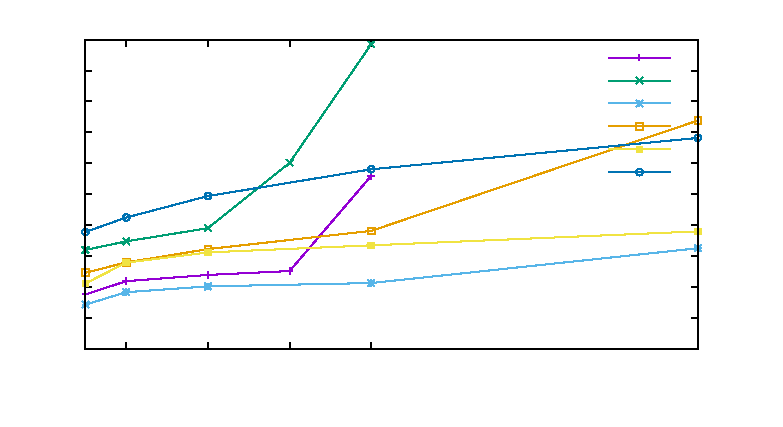
\includegraphics{readtimes2}}%
    \gplfronttext
  \end{picture}%
\endgroup

	\end{subfigure}
	\begin{subfigure}{1\textwidth}
		% GNUPLOT: LaTeX picture with Postscript
\begingroup
  \makeatletter
  \providecommand\color[2][]{%
    \GenericError{(gnuplot) \space\space\space\@spaces}{%
      Package color not loaded in conjunction with
      terminal option `colourtext'%
    }{See the gnuplot documentation for explanation.%
    }{Either use 'blacktext' in gnuplot or load the package
      color.sty in LaTeX.}%
    \renewcommand\color[2][]{}%
  }%
  \providecommand\includegraphics[2][]{%
    \GenericError{(gnuplot) \space\space\space\@spaces}{%
      Package graphicx or graphics not loaded%
    }{See the gnuplot documentation for explanation.%
    }{The gnuplot epslatex terminal needs graphicx.sty or graphics.sty.}%
    \renewcommand\includegraphics[2][]{}%
  }%
  \providecommand\rotatebox[2]{#2}%
  \@ifundefined{ifGPcolor}{%
    \newif\ifGPcolor
    \GPcolorfalse
  }{}%
  \@ifundefined{ifGPblacktext}{%
    \newif\ifGPblacktext
    \GPblacktexttrue
  }{}%
  % define a \g@addto@macro without @ in the name:
  \let\gplgaddtomacro\g@addto@macro
  % define empty templates for all commands taking text:
  \gdef\gplbacktext{}%
  \gdef\gplfronttext{}%
  \makeatother
  \ifGPblacktext
    % no textcolor at all
    \def\colorrgb#1{}%
    \def\colorgray#1{}%
  \else
    % gray or color?
    \ifGPcolor
      \def\colorrgb#1{\color[rgb]{#1}}%
      \def\colorgray#1{\color[gray]{#1}}%
      \expandafter\def\csname LTw\endcsname{\color{white}}%
      \expandafter\def\csname LTb\endcsname{\color{black}}%
      \expandafter\def\csname LTa\endcsname{\color{black}}%
      \expandafter\def\csname LT0\endcsname{\color[rgb]{1,0,0}}%
      \expandafter\def\csname LT1\endcsname{\color[rgb]{0,1,0}}%
      \expandafter\def\csname LT2\endcsname{\color[rgb]{0,0,1}}%
      \expandafter\def\csname LT3\endcsname{\color[rgb]{1,0,1}}%
      \expandafter\def\csname LT4\endcsname{\color[rgb]{0,1,1}}%
      \expandafter\def\csname LT5\endcsname{\color[rgb]{1,1,0}}%
      \expandafter\def\csname LT6\endcsname{\color[rgb]{0,0,0}}%
      \expandafter\def\csname LT7\endcsname{\color[rgb]{1,0.3,0}}%
      \expandafter\def\csname LT8\endcsname{\color[rgb]{0.5,0.5,0.5}}%
    \else
      % gray
      \def\colorrgb#1{\color{black}}%
      \def\colorgray#1{\color[gray]{#1}}%
      \expandafter\def\csname LTw\endcsname{\color{white}}%
      \expandafter\def\csname LTb\endcsname{\color{black}}%
      \expandafter\def\csname LTa\endcsname{\color{black}}%
      \expandafter\def\csname LT0\endcsname{\color{black}}%
      \expandafter\def\csname LT1\endcsname{\color{black}}%
      \expandafter\def\csname LT2\endcsname{\color{black}}%
      \expandafter\def\csname LT3\endcsname{\color{black}}%
      \expandafter\def\csname LT4\endcsname{\color{black}}%
      \expandafter\def\csname LT5\endcsname{\color{black}}%
      \expandafter\def\csname LT6\endcsname{\color{black}}%
      \expandafter\def\csname LT7\endcsname{\color{black}}%
      \expandafter\def\csname LT8\endcsname{\color{black}}%
    \fi
  \fi
    \setlength{\unitlength}{0.0500bp}%
    \ifx\gptboxheight\undefined%
      \newlength{\gptboxheight}%
      \newlength{\gptboxwidth}%
      \newsavebox{\gptboxtext}%
    \fi%
    \setlength{\fboxrule}{0.5pt}%
    \setlength{\fboxsep}{1pt}%
\begin{picture}(7200.00,3880.80)%
    \gplgaddtomacro\gplbacktext{%
      \csname LTb\endcsname%%
      \put(528,686){\makebox(0,0)[r]{\strut{}$0$}}%
      \put(528,1111){\makebox(0,0)[r]{\strut{}$20$}}%
      \put(528,1536){\makebox(0,0)[r]{\strut{}$40$}}%
      \put(528,1961){\makebox(0,0)[r]{\strut{}$60$}}%
      \put(528,2385){\makebox(0,0)[r]{\strut{}$80$}}%
      \put(528,2810){\makebox(0,0)[r]{\strut{}$100$}}%
      \put(528,3235){\makebox(0,0)[r]{\strut{}$120$}}%
      \put(528,3660){\makebox(0,0)[r]{\strut{}$140$}}%
      \put(660,554){\rotatebox{-45}{\makebox(0,0)[l]{\strut{}8192}}}%
      \put(1500,554){\rotatebox{-45}{\makebox(0,0)[l]{\strut{}16384}}}%
      \put(3180,554){\rotatebox{-45}{\makebox(0,0)[l]{\strut{}32768}}}%
      \put(6119,554){\rotatebox{-45}{\makebox(0,0)[l]{\strut{}61440}}}%
      \put(6539,554){\rotatebox{-45}{\makebox(0,0)[l]{\strut{}65536}}}%
    }%
    \gplgaddtomacro\gplfronttext{%
      \csname LTb\endcsname%%
      \put(5552,3487){\makebox(0,0)[r]{\strut{}readtimes-by-array-size-desktop}}%
      \csname LTb\endcsname%%
      \put(5552,3267){\makebox(0,0)[r]{\strut{}readtimes-by-array-size-padded-desktop}}%
      \csname LTb\endcsname%%
      \put(5552,3047){\makebox(0,0)[r]{\strut{}readtimes-by-array-size-server}}%
      \csname LTb\endcsname%%
      \put(5552,2827){\makebox(0,0)[r]{\strut{}readtimes-by-array-size-padded-server}}%
    }%
    \gplbacktext
    \put(0,0){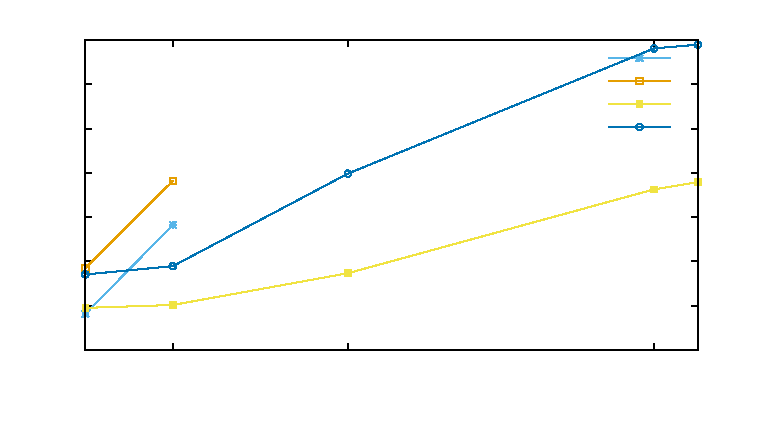
\includegraphics{readtimes3}}%
    \gplfronttext
  \end{picture}%
\endgroup

	\end{subfigure}
	\caption{Random cyclic reads. The average read time measured over
	$2^{25}$ reads as a function of the working-set size in bytes. \mynote{I
	should adjust the colors so they are consistent across plots, and maybe
	remove the legends}}
	\label{fig:readtimes}
\end{figure}
